% !TEX root = ../thesis.tex
\chapter{Prototype validation}
\label{sec:validation}

To validate the architecture described in the thesis, we carried out several tests aimed at both testing the functionalities implemented, and to measure the performance of the infrastructure layer in terms of throughput, latency introduced and resource required.
%The tests were repeated both with an infrastructure layer consisting of a single integrated node, as well as in case of an OpenStack cluster composed by two compute nodes.
%in case it consists of two servers under the same OpenStack domain.
%Note that, in the latter case the graphs are split so that the VNFs are distributed between the two physical servers.
\begin{comment}
Moreover, during the tests the end users are connected to the infrastructure through a common wireless interface, while their SGs are cascaded to a common graph defined by the ISP and that provides connectivity to the Internet, as depicted in Figure~\ref{fig:deployed_graphs}. 
\end{comment}

\section{Service overview}

The FGs deployed in the tests are shown in Figure~\ref{fig:deployed_graphs}; according to our use case implementation, these graphs include the authentication graph used to authenticate new end users connected to the network, and the ISP graph, which provides connectivity to the Internet and is crossed by the traffic generated from/going towards all the end users.
The control network of this ISP graph  also includes a firewall, so that only the authorized entities (e.g., the ISP itself) can control and configure the deployed VNFs.

\begin{figure}%[h]
	\centering
	% left bottom right top
	\includegraphics[clip= true, width= 0.8\columnwidth, trim= 0in 0.2in 0.0in 0.6in, page= 29]{images/Pictures_definitivo.pdf}
	\caption{Use case scenario.}
	\label{fig:deployed_graphs}
\end{figure}

As evident from the picture, each end user graph provides an example of traffic steering, since it requires that the packets towards the Internet is split so that the web traffic is provided to a traffic monitor and then to a firewall that blocks the HTTP GET towards specific URLs, while the other packets simply traverse a second traffic monitor VNF.
It is worth noting that, thanks to the control interface of the traffic monitors we are able to observe the packets flowing through the specific VNF, and hence to validate the correct behavior of the traffic steering mechanism.

During the tests carried out on the OpenStack-based node, the VNFs are implemented as VMs running on the KVM hypervisor and in a second OpenStack-based node VNFs are implemented in Docker containers.
Instead, in the tests with the integrated node, the firewall is implemented as a DPDK process, while all the others VNFs are implemented in Docker containers.
In particular, both the VMs and the Docker containers run an Ubuntu operating system, and the VNFs are implemented through \textit{standard} Linux tools (e.g., iptables).


As a final remark, according to our use case and the current implementation of the architecture, the end users are directly connected to the node on which their graphs are deployed. %; \textit{(ii)} the user graphs are cascaded to a common graph defined by the ISP and that provides connectivity to the Internet, as depicted in Figure~\ref{fig:deployed_graphs}. 

\section{Performance evaluation}
This section shows the tests executed in order to measure the performance obtained with the preliminary implementation of our architecture.

During the tests, a machine is dedicated to the execution service layer (i.e., service layer application, Keystone) and the global orchestrator; it is equipped with 16 GB RAM, 500GB HD, Intel i7-2620M @ 2.7 GHz (one core plus hyperthreading) and OSX 10.9.5, Darwin Kernel Version 13.4.0, 64 bit, which is the same for both the infrastructure nodes.

The infrastructure layer is implemented on a set of servers with 32 GB RAM, 500GB HD, Intel i7-3770 @ 3.40 GHz CPU (four cores plus hyperthreading) and Ubuntu 12.04 server OS, kernel 3.11.0-26-generic, 64 bits.
In case of OpenStack-based node, a first machine hosts the infrastructure controller (Heat, Nova scheduler, Nova API, Neutron and ODL), the network node, while another one is dedicated to the implementation of the Nova compute node, connected through a Gigabit Ethernet link. In addition to the nova compute that runs VMs another one node, that runs Docker container, is connected in the same OpenStack domain.
%In case of OpenStack-based node, a first machine hosts the infrastructure controller (Heat, Nova scheduler, Nova API, Neutron and ODL), the network node, as well as it acts as a Nova compute node, while another one is dedicated to the implementation of the second Nova compute node, connected through a Gigabit Ethernet link.
In case of the integrated node, one of those machines executes all the software.

The memory required by the different components of the system is reported in Table~\ref{tab:memory}, in which the consumption related to the Nova compute node and to the integrated node has been measured without any VNF deployed.


\renewcommand{\arraystretch}{1.5}
\begin{table*}[htbp]
	\centering
	\tiny
	\caption{Memory consumption.}
	\label{tab:memory}
	\begin{tabular}{c|c}
		%\toprule
		\textbf{Component} & \textbf{Memory [MB]} \\
		\hline	
		\hline
		Service layer + global orchestrator & \\
		(SLApp + Keystone + Horizon + & 558.2\\
		additional (minor) libraries/components)  & \\
		\hline
		Infrastructure controller & \\
		(Heat + Nova scheduler + Nova API + Neutron + ODL + & 3396.7\\
		additional (minor) libraries/components) &  \\
		\hline
		Nova compute node & \\
		(Nova compute + OVS +  & 294.8\\
		additional (minor) libraries/components) &  \\
		\hline
		Integrated node & 120.5\\
		(node resource manager + xDPd + additional (minor) libraries) & \\
		\hline 
		%	\bottomrule
	\end{tabular}
\end{table*}

As evident, the infrastructure controller for the OpenStack-based node is the heaviest component, while the requirements of the integrated node, which is almost based on ad hoc modules, is quite reduced.




\subsection{Deployment time}
%The conditions in that we repeated the tests is the follow: \textit{(i)} user device and server directly connected using a gigabit Ethernet link; \textit{(ii)} user devices connected, through a gigabit Ethernet network, to the node on which the graphs are deployed, which is in turn connected to the server through gigabit Ethernet link.
%Moreover, as node running the VNFs, we used:  an OpenStack-based node with a single server that runs VMs,  an OpenStack-based node consisting of two servers connected with a gigabit Ethernet link VMs, an OpenStack-based node with a single server that runs docker, and the integrated node.

The first kind of tests performed is concerned about the measuring of service deployment time. The table~\ref{tab:fg_istatiatiotion_evaluation}
shows the times of instantiation of the user service graph detailed before, and the transitory time between the instantiation of the graph and the time in which the user is able to ping the server. It also shows the total time of the SG deployment, as we can see, those times are anything but low. What appears to be obvious looking at the Table~\ref{tab:fg_istatiatiotion_evaluation} is that, the imputable for those results is the infrastructure layer, which is in charge of both VMs/dockers instantiation and the creation of paths between them.
It is worth pointing out that this time does not include the download of the VNF images from the repository, which are already cached on the physical nodes.
%
\renewcommand{\arraystretch}{1.5}
\begin{table*}[htbp]
	\centering
	\tiny
	\caption{Deployment time.}
	\label{tab:fg_istatiatiotion_evaluation}
	\begin{tabular}{c|c|c|c|c|c}
		%\toprule
		\textbf{Component} & Service layer & Global orchestrator & Infrastructure layer & Ping & \textbf{Tot} \\
		\hline	
		\hline

		Openstack single node & 0.83 & 0.61 & 127 & 49 & 177.44\\
		(virtual machine)  & & & & & \\
		\hline

		%Openstack two nodes & X & X & 132 & 183 & X\\
		%(virtual machine) & & & & & \\
		%\hline

		Openstack sigle node  & 0.83 & 0.61 & 82 & 13 & 96.44\\
		(docker) & & & & &\\
		\hline
		% SLApp + orch = 1.32
		Integrated node & 0.83 & 0.49 & 72.67 & 11 & 84.99\\
		
		\hline 
		%	\bottomrule
	\end{tabular}
\end{table*}

This test has been repeated using different graphs with a variable number of VNFs and the results are shown in Figure~\ref{fig:startup_times}. All the VNFs use the same image, and all nodes used for the test have it stored locally. One OpenStack node uses VMs that run an Ubuntu Server 12.04 and the size of the image is 1.6 GB. The other one OpenStack node and the integrated node use the Docker containers that run an Ubuntu Server 12.04 and the size of the image is 0.324 GB. Furthermore, in both VMs and Docker containers are used linux bridges to forward of traffic between the vNICs. In these tests the ping time is not considered. Hence, this means that after the time shown in Figure~\ref{fig:startup_times} the user is not immediately able to access to his service. Indeed, as we can see looking the ping value in Table~\ref{tab:fg_istatiatiotion_evaluation}, especially in OpenStack with VMs, the time for starting the services is very high.
%
\begin{figure}[H]
	\centering
	% left bottom right top
	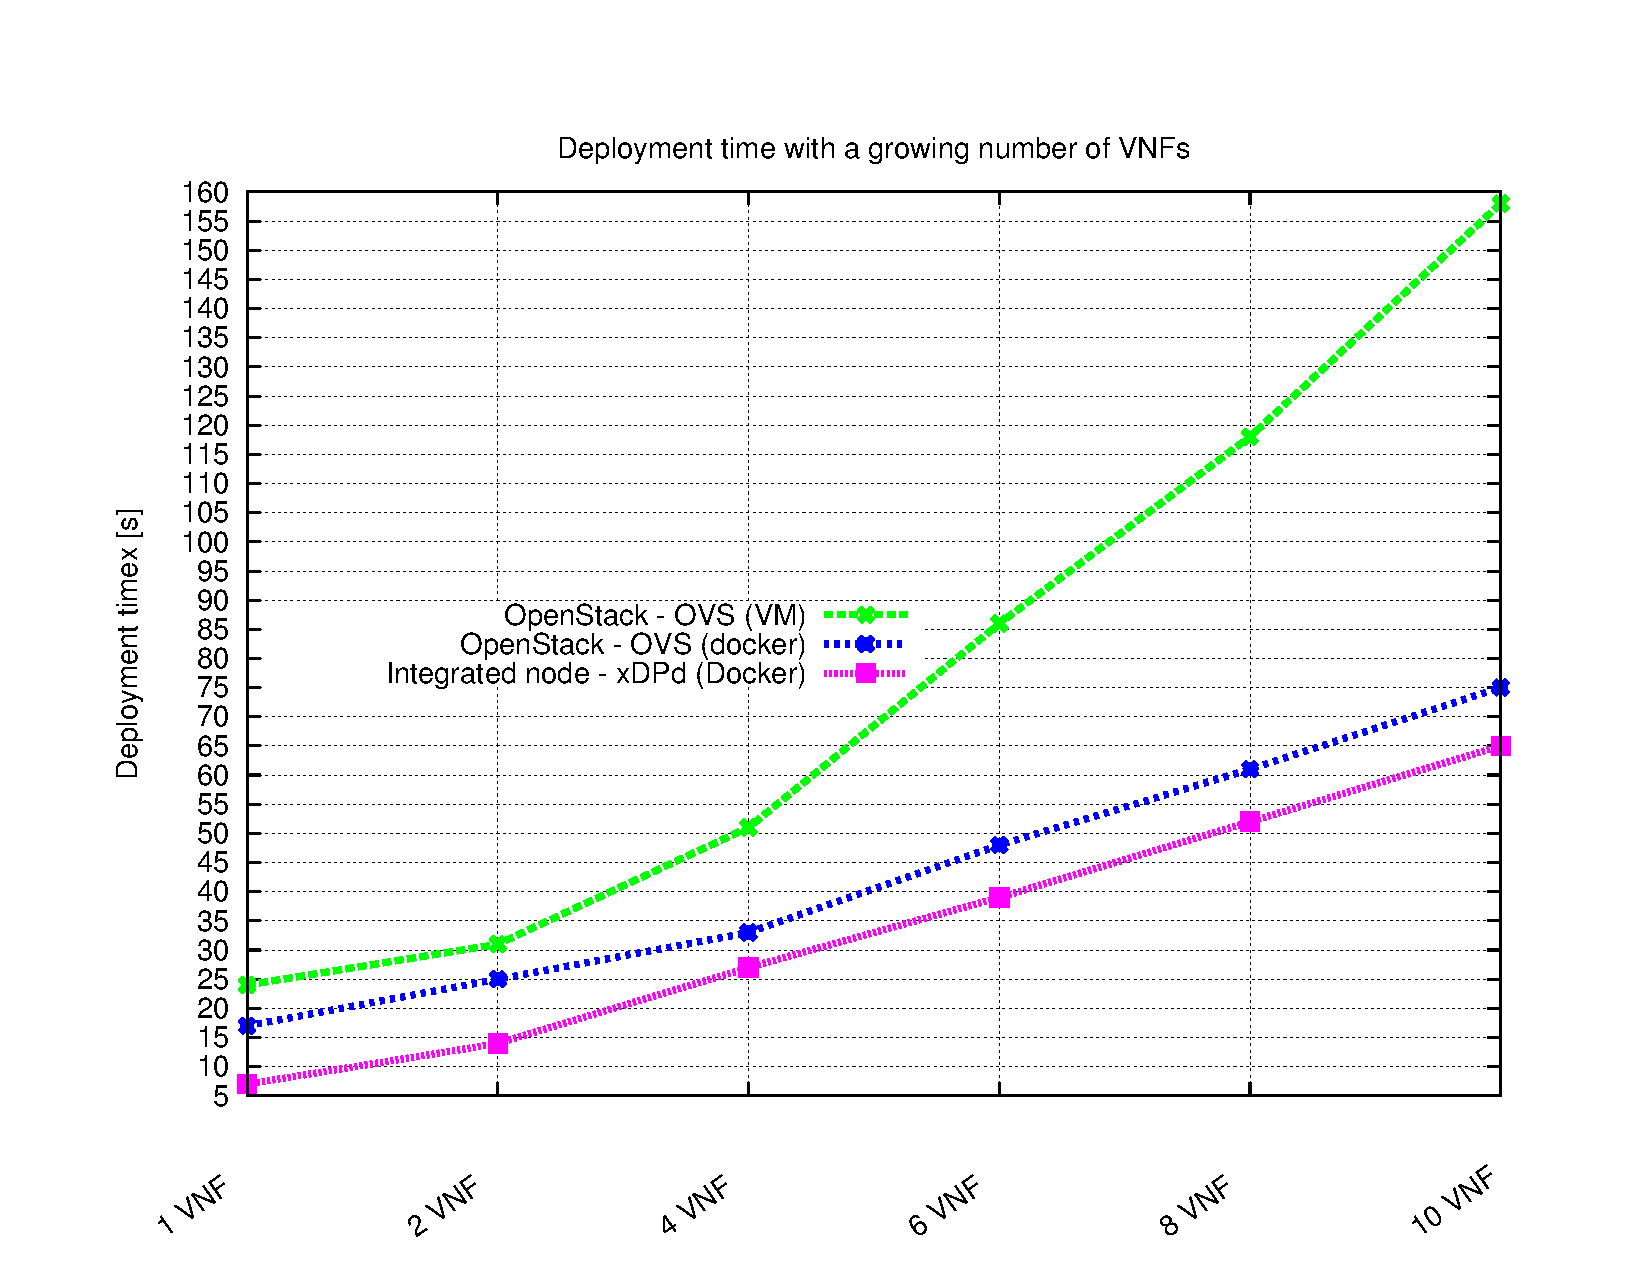
\includegraphics[clip= true, width=0.5\columnwidth]{images/graphs/startup_times.pdf}
	\caption{Startup times.}
	\label{fig:startup_times}
\end{figure}
%
Anyway these performance show a behavior almost linear according to a growing number of VNFs.






\subsection{Throughput and latency}

The second phase of performance evaluation has been dedicated to analyze the throughput that we can achieve on the different infrastructure layers. As shown on the left of the Table~\ref{tab:evaluation}, the different infrastructure layers used are \textit{(i)} OpenStack-based node that runs virtual machines, \textit{(ii)}  OpenStack-based node that runs Docker container, and \textit{(iii)} the integrated node. Also the tests of Figure~\ref{tab:evaluation} are performed connecting directly the user and the server machine. %As shown in Table~\ref{tab:evaluation}, we repeated the tests in the following conditions: \textit{(i)} user device and server directly connected using a gigabit Ethernet link; \textit{(ii)} user devices connected, through a gigabit Ethernet network, to the node on which the graphs are deployed, which is in turn connected to the server through gigabit Ethernet link.
%Moreover, as node running the VNFs, we used: an OpenStack-based node that using VMs, an OpenStack-based node that using VMs, the integrated node.
The first test carried out aims at measuring the latency introduced by the deployed services (Figure~\ref{fig:deployed_graphs}); in particular, the user device(s) sends 100 \texttt{ping} towards the server, and the results were averaged and reported in the left part of the table.
%\footnote{It is worth noting that, according to the deployed SGs, packets exchanged in this test are not handled by the firewall VNF, which only operates on HTTP traffic.}.
The second and third tests are made on TCP traffic so they are most interested about perception of quality of service by end user. In particular the second test aimed at measuring throughput obtained during the download of a file of 4 GB from the server, and it is performed using  \texttt{wget}, a Linux tool that uses the HTTP protocol. Whilst the third test is done using \texttt{iperf}, a network testing tool that can create TCP and UDP data streams and measure the throughput of a network that is carrying them. Finally, the last test is performed for evaluate the performance on UDP traffic, even in this case has been used \texttt{iperf}.
As a consequence, according to the user graph, while the ping are not handled by the firewall, this VNF is instead involved during the file transfer.
%
%
\renewcommand{\arraystretch}{1.5}
\begin{table*}[!htbp]
	\centering
	\tiny
	\caption{Performance of the infrastructure layer.}
	\label{tab:evaluation}
	\begin{tabular}{l||c|c|c|c||}
		%\toprule
		%\multirow{2}{*}{\textbf{Attack settings}} & 
		& \textbf{Ping (avg) } & \textbf{File transfer (wget) }& \textbf{TCP test (iperf)}  & \textbf{UDP test (iperf)}\\ & \textbf{[ms]} & \textbf{[Mbps]} & \textbf{[Mbps]} & \textbf{[Mbps]}\\
		
		\hline	
		\hline
		\textbf{\#1 Direct connection} & 0.41  & 864  & 934  & 810 \\
		\hline
		\textbf{\#2 OS compute node - VMs (i7)} & 3.33  & 770.4 & 841 & 779 \\
		\hline
		%	\midrule
		%	\midrule
		\textbf{\#3 OS one compute node - docker (i7)} & 0.71 & 795.2  & 932 & 761   \\
		%	\midrule
		\hline
		\textbf{\#4 Integrated node (i7)} & 62.04 & 210.4 & 247  & 410\\
		\hline
		%	\bottomrule
	\end{tabular}
\end{table*} 

Furthermore all performance tests have been repeated using graphs with a variable number of VNFs, as done for evaluating the deployment time. The results are shown in Figure~\ref{fig:performance_tests}.

\begin{figure*}%[ht]
	\begin{center}
		\subfloat[Round trip time.]{%
			\label{fig:end_test1}
			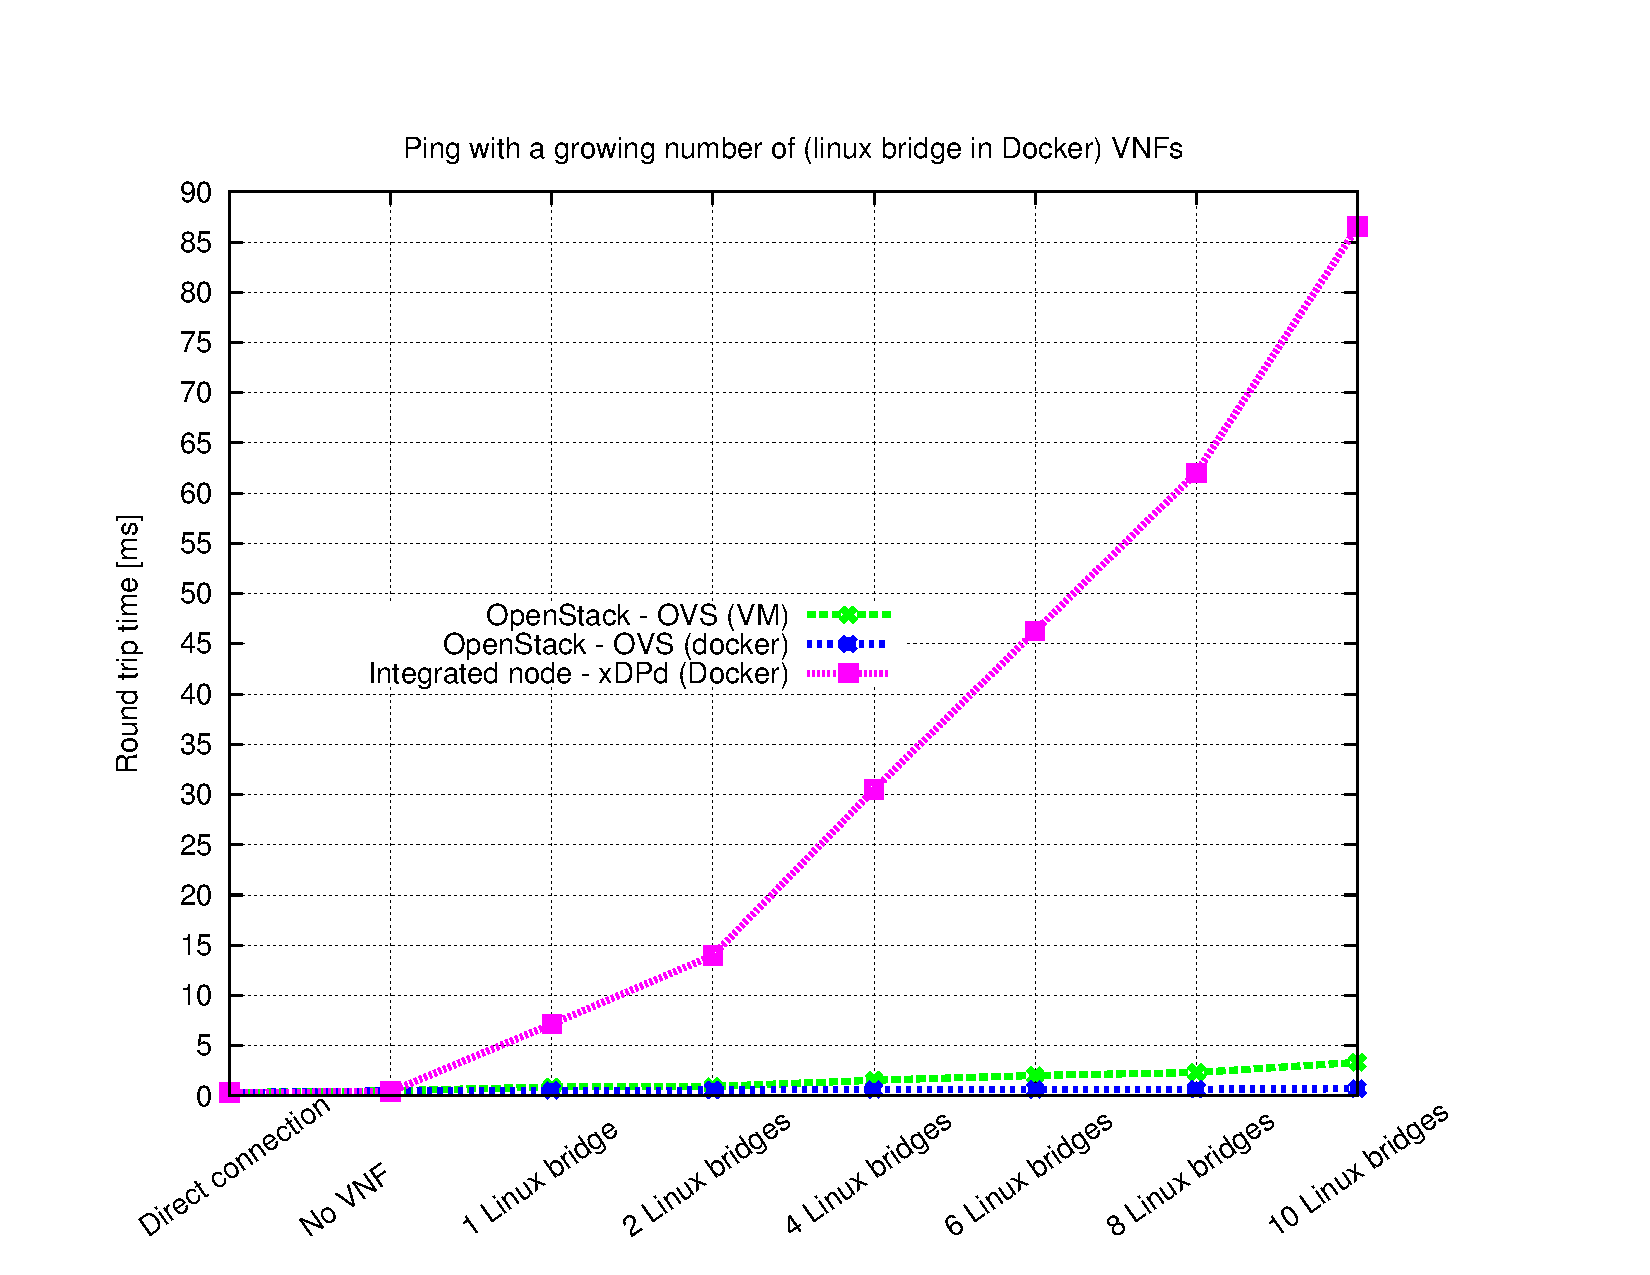
\includegraphics[clip= true, width= 0.5\columnwidth]{images/graphs/ping.pdf}
		}%
		\subfloat[Througput TCP - \textit{wget}.]{%
			\label{fig:end_test2}
			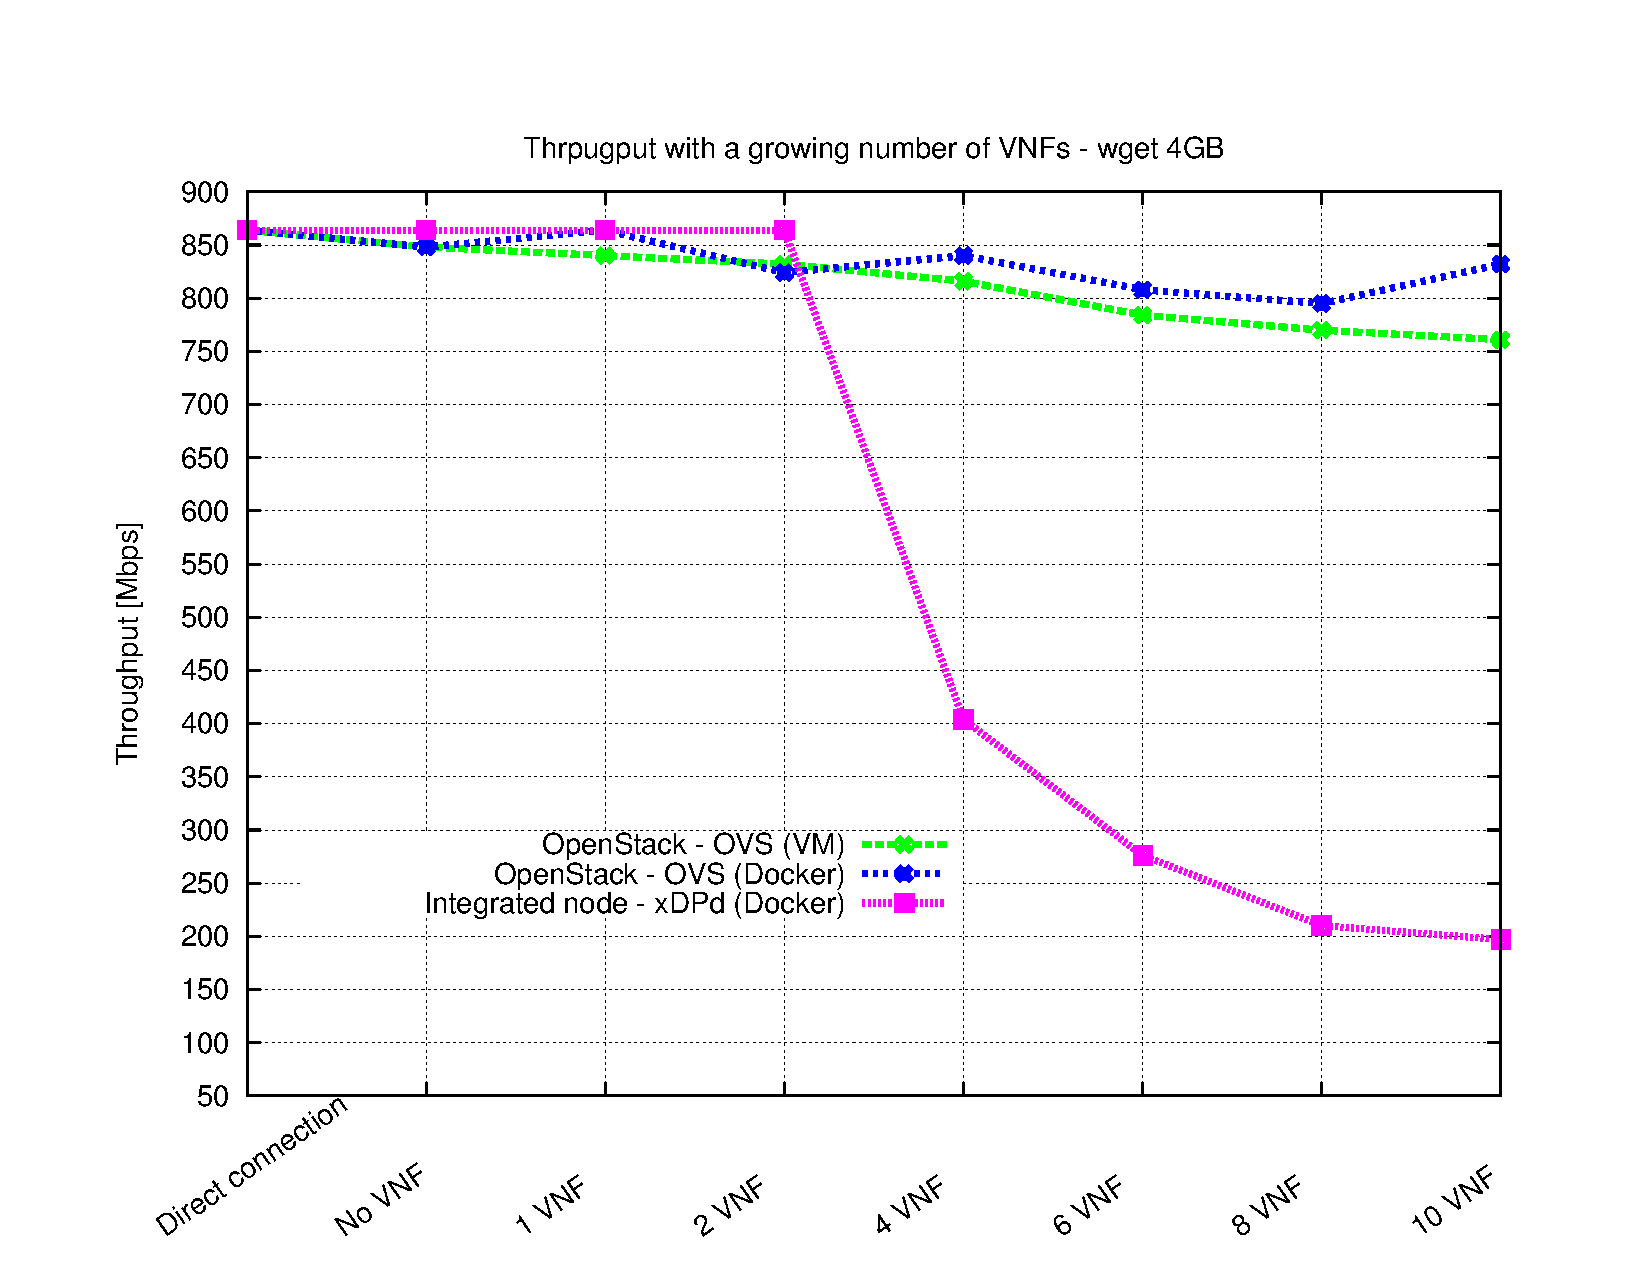
\includegraphics[clip= true, width= 0.5\columnwidth]{images/graphs/tcp_wget_throughput.pdf}
		}\\ %  ------- End of the first row ----------------------%
		\subfloat[Througput TCP - \textit{iperf}.]{%
			\label{fig:end_test3}
			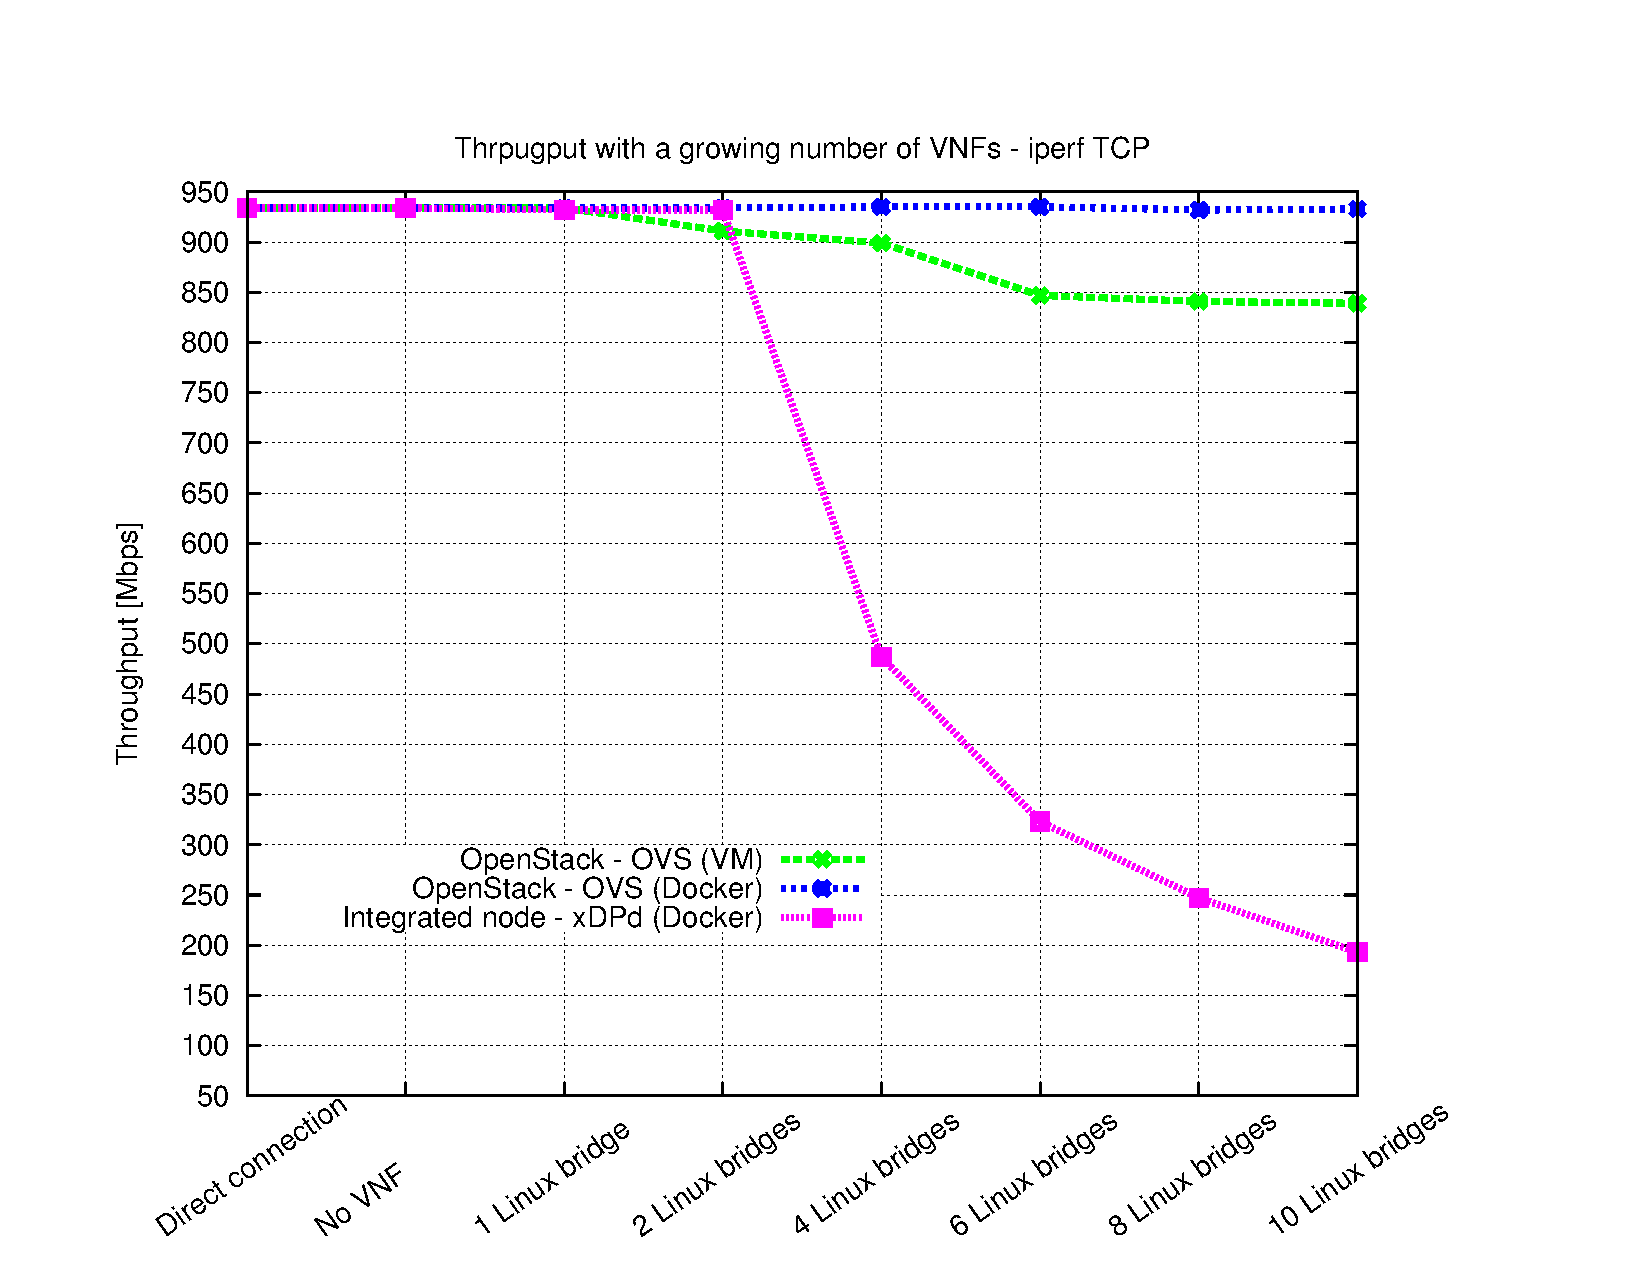
\includegraphics[clip= true, width= 0.5\columnwidth]{images/graphs/tcp_iperf_throughput.pdf}
		}%
		\subfloat[Througput UDP - \textit{iperf}.]{%
			\label{fig:end_test4}
			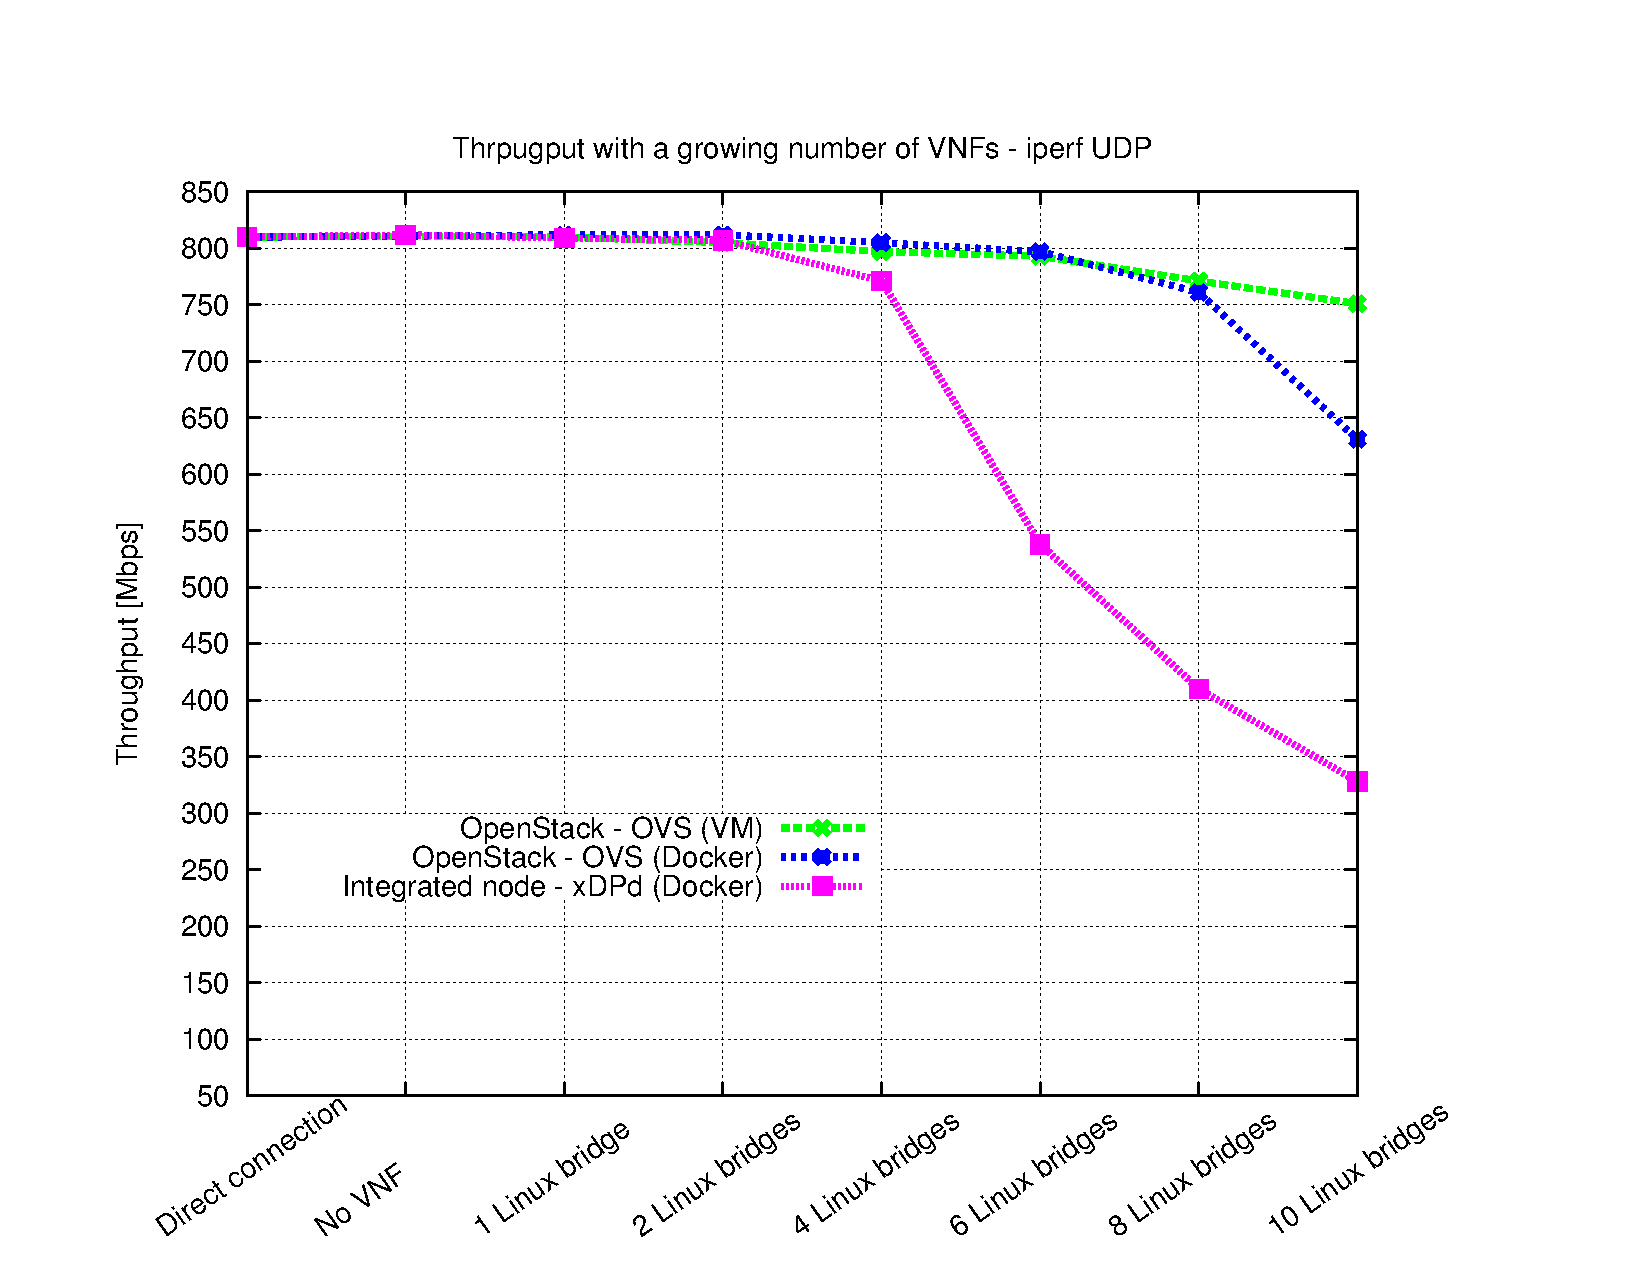
\includegraphics[clip= true, width= 0.5\columnwidth]{images/graphs/udp_throughput.pdf}
		}%
	\end{center}
	\caption{Performance tests. }
	\label{fig:performance_tests}
\end{figure*}

As expected, the deployment of a SG on the network does not come for free, since the results obtained are lower with respect to the case in which no service is instantiated between the user device and the server.
However, as evident by a comparison between line \texttt{\#1}, \texttt{\#2} and \texttt{\#3} of the table, this penalty is limited when the graph is deployed on an OpenStack-based node that use VMs, and almost zero when we use an OpenStack-based node using Docker containers.

Instead, when the user graph is scheduled in the integrated node (line \texttt{\#4}), performance are worse in all tests evaluated.

